\documentclass[12pt,a4paper]{article}

% ============================================================================
% PACKAGES
% ============================================================================
\usepackage[utf8]{inputenc}
\usepackage[T1]{fontenc}
\usepackage{lmodern}
\usepackage[margin=2.8cm]{geometry}
\usepackage{amsmath,amssymb}
\usepackage{xcolor}
\usepackage{tikz}
\usepackage{hyperref}
\usepackage{fancyhdr}
\usepackage{titlesec}
\usepackage{lettrine}
\usepackage{setspace}
\usepackage{parskip}
\usepackage{epigraph}
\usepackage{enumitem}
\usepackage{microtype}
\usepackage{graphicx}
\usepackage{abstract}

% ============================================================================
% CONFIGURATION
% ============================================================================
\usetikzlibrary{decorations.pathmorphing, decorations.markings, arrows.meta, calc, patterns, fadings}

% Colors
\definecolor{voidblack}{RGB}{10, 10, 20}
\definecolor{deepblue}{RGB}{20, 60, 120}
\definecolor{quantumblue}{RGB}{70, 130, 200}
\definecolor{starwhite}{RGB}{255, 255, 240}
\definecolor{nebula}{RGB}{150, 100, 180}
\definecolor{fieldgreen}{RGB}{80, 180, 140}
\definecolor{amber}{RGB}{200, 150, 50}
\definecolor{cosmicred}{RGB}{180, 60, 60}
\definecolor{fluxcyan}{RGB}{0, 200, 220}
\definecolor{galaxypurple}{RGB}{120, 60, 200}

\hypersetup{
    colorlinks=true,
    linkcolor=deepblue,
    citecolor=nebula,
    urlcolor=quantumblue,
    pdftitle={The Cosmic Flux: Stars, Galaxies, and the Universe as a Distributed Consensus Machine},
    pdfauthor={Q-NarwhalKnight Research Group}
}

% Header/Footer
\pagestyle{fancy}
\fancyhf{}
\fancyhead[LE,RO]{\small\thepage}
\fancyhead[RE]{\small\textit{The Cosmic Flux}}
\fancyhead[LO]{\small\textit{Q-NarwhalKnight Philosophy}}
\renewcommand{\headrulewidth}{0.4pt}

% Title formatting
\titleformat{\section}{\Large\bfseries\color{deepblue}}{\thesection}{1em}{}[\vspace{-0.5em}\color{deepblue}\rule{\textwidth}{0.3pt}]
\titleformat{\subsection}{\large\bfseries\color{nebula}}{\thesubsection}{1em}{}
\titleformat{\subsubsection}{\normalsize\itshape\color{amber}}{\thesubsubsection}{1em}{}

\setstretch{1.4}
\setlength{\epigraphwidth}{0.75\textwidth}
\setlength{\epigraphrule}{0pt}

% ============================================================================
% DOCUMENT
% ============================================================================
\begin{document}

\begin{titlepage}
\begin{center}
\vspace*{1cm}

% Decorative cosmic TikZ header

\begin{tikzpicture}[remember picture, overlay]
    \fill[voidblack] (current page.north west) rectangle (current page.south east);
    % Stars
    \foreach \i in {1,...,200}{
        \pgfmathsetmacro{\x}{rand*10}
        \pgfmathsetmacro{\y}{rand*14}
        \pgfmathsetmacro{\r}{0.01 + rand*0.03}
        \fill[white, opacity={0.3 + rand*0.7}] (\x, \y-7) circle (\r);
    }
    % Galaxy spiral
    \foreach \a in {0,5,...,720}{
        \pgfmathsetmacro{\r}{0.3 + \a/300}
        \pgfmathsetmacro{\x}{\r*cos(\a)}
        \pgfmathsetmacro{\y}{\r*sin(\a)}
        \pgfmathsetmacro{\opac}{0.8 - \a/1000}
        \fill[galaxypurple, opacity=\opac] (\x, \y+2) circle (0.04);
    }
    % Another spiral arm
    \foreach \a in {0,5,...,720}{
        \pgfmathsetmacro{\r}{0.3 + \a/300}
        \pgfmathsetmacro{\x}{\r*cos(\a+180)}
        \pgfmathsetmacro{\y}{\r*sin(\a+180)}
        \pgfmathsetmacro{\opac}{0.8 - \a/1000}
        \fill[fluxcyan, opacity=\opac] (\x, \y+2) circle (0.04);
    }
    % Bright center
    \fill[starwhite, opacity=0.9] (0, 2) circle (0.15);
    \fill[fluxcyan, opacity=0.3] (0, 2) circle (0.5);
\end{tikzpicture}

\vspace{2cm}

\includegraphics[width=5cm]{flux_logo}

\vspace{1cm}

{\fontsize{28}{34}\selectfont\bfseries\color{starwhite} The Cosmic Flux}\\[0.5cm]
{\fontsize{16}{20}\selectfont\color{fluxcyan} Stars, Galaxies, and the Universe\\as a Distributed Consensus Machine}\\[1cm]
{\large\color{starwhite} A Philosophical Expedition into Why Everything That Spins,\\Shines, and Streams Is Basically Running the Same Protocol}

\vspace{2cm}

{\color{amber}\large Q-NarwhalKnight Research Group}\\[0.3cm]
{\color{nebula} Philosophy \& Cosmology Division}\\[0.5cm]
{\color{starwhite}\small March 2026}\\[0.3cm]
{\color{fluxcyan}\small\texttt{v1.0 --- Peer Review Welcome}}

\vspace{1cm}

{\color{starwhite}\small
\textit{``The universe is not only queerer than we suppose,}\\
\textit{but queerer than we \emph{can} suppose.''}\\
\vspace{0.2cm}
--- J.B.S. Haldane (who clearly never tried debugging a distributed system)}
\end{center}
\end{titlepage}

% ============================================================================
\begin{abstract}
\noindent
We present a philosophical framework arguing that the observable universe
operates as a naturally-occurring distributed consensus system. Stars are
worker nodes, galaxies are sharded clusters, photons are gossip protocol
messages, and gravity is the ultimate Byzantine fault tolerance mechanism.
We demonstrate (with varying degrees of seriousness) that every problem
solved by modern reverse proxies --- load balancing, TLS termination,
connection pooling, backpressure, and graceful shutdown --- was first solved
by the cosmos approximately 13.8 billion years ago. We introduce the concept
of \textbf{Cosmic Flux}: the idea that information, energy, and consensus
flow through the universe in the same worker-per-core pattern that makes
high-performance networking possible. We conclude that building software
is really just the universe becoming aware of its own architecture.
\end{abstract}

\tableofcontents
\newpage

% ============================================================================
\section{Introduction: The Universe Had the Idea First}
% ============================================================================

\lettrine[lines=3, loversize=0.15]{\color{galaxypurple}E}{very} programmer who has
ever written a load balancer has, without knowing it, been engaged in an act of
cosmic plagiarism. The universe invented distributed systems 13.8 billion years
before the first RFC was drafted. It invented sharding before databases existed.
It invented eventual consistency before anyone thought to give it a name.

Consider the Milky Way galaxy. It contains approximately 200 billion stars, each
one a fusion reactor running its own local consensus on what temperature to be.
These stars do not need a coordinator. There is no Central Star Authority issuing
certificates. Each star simply follows the laws of physics --- the original protocol
specification --- and from this local adherence emerges the grand spiral structure
that we see when we look up on a clear night.

\epigraph{\textit{``In the beginning there was nothing. Then there was a gossip
protocol, and it was good.''}}{\textsc{--- The Book of Distributed Genesis, 1:1}}

This paper argues that the architectural patterns we celebrate in modern
high-performance networking --- worker-per-core execution, SO\_REUSEPORT
kernel-level distribution, zero-contention connection pooling, TLS-like
handshakes, and graceful shutdown with drain timeouts --- are not inventions.
They are \emph{discoveries}. The universe has been running these patterns
since the first photon propagated through the primordial plasma. We are merely
writing them down in Rust.

% ============================================================================
\section{Stars as Worker Nodes}
% ============================================================================

\subsection{The Main Sequence as a Process Model}

A star on the main sequence is the universe's version of a worker thread pinned
to a specific core. It has:

\begin{itemize}[leftmargin=2cm]
    \item[\color{amber}$\star$] \textbf{Dedicated resources}: Its own gravitational
    well, its own fuel supply, its own radiation budget. No sharing with neighbors.
    Zero contention on the hot path.

    \item[\color{amber}$\star$] \textbf{Local state}: Temperature, luminosity,
    metallicity --- all maintained locally without consulting a central database.

    \item[\color{amber}$\star$] \textbf{Bounded lifetime}: Stars don't run forever.
    They have a drain timeout. When hydrogen runs out, they go through a graceful
    shutdown sequence (red giant phase, planetary nebula ejection, white dwarf
    cooling). The most dramatic stars skip graceful and go straight to
    \texttt{kill -9} (supernova).

    \item[\color{amber}$\star$] \textbf{Output streaming}: Stars continuously emit
    photons --- the universe's equivalent of Server-Sent Events. Every star is an
    SSE endpoint that has been streaming for billions of years without a single
    \texttt{503 Service Unavailable}.
\end{itemize}

\subsection{SO\_REUSEPORT: The Gravitational Version}

When multiple processes bind to the same port with \texttt{SO\_REUSEPORT}, the
Linux kernel distributes incoming connections across them fairly, with no
thundering herd. Stars in a globular cluster achieve the same effect. Incoming
photons from distant galaxies arrive at the cluster, and each star captures
photons proportional to its cross-section. No coordinator required. The
``kernel'' here is general relativity.

\begin{center}
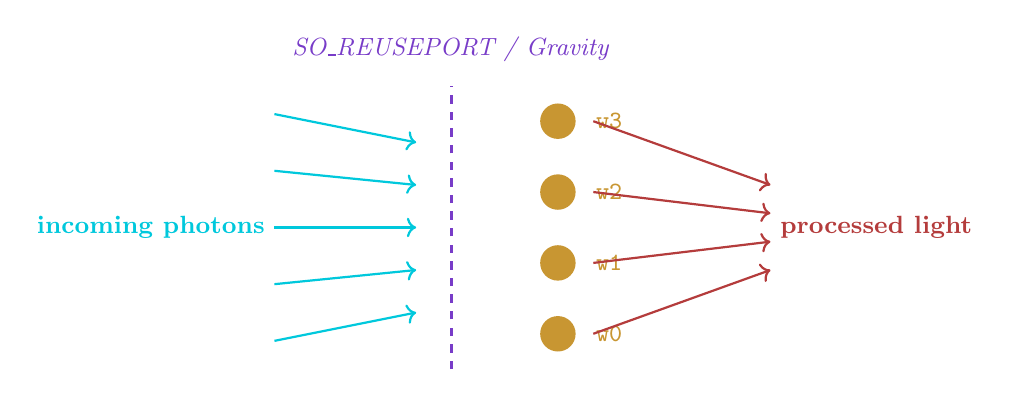
\begin{tikzpicture}[scale=0.9]
    % Incoming photons
    \foreach \y in {-2,-1,0,1,2} {
        \draw[->, fluxcyan, thick] (-4, \y*0.8) -- (-2, \y*0.6);
    }
    \node[fluxcyan, left] at (-4, 0) {\small\textbf{incoming photons}};

    % Stars (workers)
    \foreach \y/\name in {-1.5/w0, -0.5/w1, 0.5/w2, 1.5/w3} {
        \fill[amber] (0, \y) circle (0.25);
        \node[right, amber] at (0.4, \y) {\small\texttt{\name}};
    }

    % Kernel distribution
    \draw[dashed, galaxypurple, thick] (-1.5, -2) -- (-1.5, 2);
    \node[galaxypurple, above] at (-1.5, 2.2) {\small\textit{SO\_REUSEPORT / Gravity}};

    % Output
    \foreach \y in {-1.5,-0.5,0.5,1.5} {
        \draw[->, cosmicred, thick] (0.5, \y) -- (3, \y*0.4);
    }
    \node[cosmicred, right] at (3, 0) {\small\textbf{processed light}};
\end{tikzpicture}
\end{center}

% ============================================================================
\section{Galaxies as Sharded Clusters}
% ============================================================================

If stars are worker threads, then galaxies are sharded database clusters. Each
galaxy maintains its own local state (stars, gas, dark matter), processes its
own transactions (stellar births, supernovae, mergers), and communicates with
other galaxies only through a slow, high-latency gossip protocol
(electromagnetic radiation traveling at \emph{c}).

\subsection{The Latency Problem}

The Andromeda galaxy is 2.537 million light-years away. If you sent a
\texttt{GET /api/v1/status} request to Andromeda right now, you would
receive the response in 5.074 million years. This is, to put it mildly,
worse than the average API timeout. Yet the universe handles this gracefully
through \textbf{eventual consistency}. Andromeda does not need to know our
current state to function. It maintains its own local consensus, and the
two galaxies will eventually merge their state (literally, in about
4.5 billion years, in what cosmologists call the ``Milkomeda merger''
and what engineers would call a ``database migration from hell'').

\subsection{Dark Matter: The Ultimate Load Balancer}

Dark matter constitutes approximately 85\% of the mass of the universe
and does exactly one thing: it provides gravitational scaffolding that
determines where galaxies form and how they distribute themselves.
It is the universe's nginx --- invisible, unglamorous, absolutely essential,
and responsible for routing 85\% of all traffic without anyone seeing it do
any work.

Unlike nginx, dark matter has never crashed, never leaked goroutines,
and never consumed 7.1 GB of RAM after six minutes of operation. We
aspire to this level of reliability.

% ============================================================================
\section{Photons as Gossip Protocol Messages}
% ============================================================================

\subsection{The Speed of Light as Bandwidth Limit}

Every photon emitted by every star is a gossip message. It carries information
about the star's state: temperature (frequency), intensity (amplitude), chemical
composition (absorption lines). This information propagates at the maximum
bandwidth of the universe --- the speed of light, $c = 299{,}792{,}458$ m/s.

Photons are the universe's \texttt{/qnk/mainnet2026.1/blocks} topic. Every
node (star) publishes to this topic continuously, and every other node that
can ``see'' it receives the message. The propagation is:

\begin{itemize}
    \item \textbf{One-to-many}: A single photon emission radiates in all directions.
    \item \textbf{Eventually delivered}: Given enough time, every photon reaches
    every point in its future light cone.
    \item \textbf{Immutable}: Once emitted, a photon's state cannot be altered.
    It is the ultimate append-only log.
    \item \textbf{Ordered by arrival}: Observers see photons in the order they
    arrive, not the order they were emitted. This is literally how SSE works.
\end{itemize}

\subsection{TLS: The Cosmic Version}

When two particles interact for the first time, they must establish a shared
reference frame. This is the physics equivalent of a TLS handshake:

\begin{enumerate}
    \item \textbf{ClientHello}: Photon arrives at atom, presenting its wavelength
    and polarization.
    \item \textbf{ServerHello}: Atom checks if the photon's energy matches an
    available electron transition (certificate validation).
    \item \textbf{Key Exchange}: If the energy matches, the photon is absorbed
    and a new photon may be re-emitted (session established).
    \item \textbf{Handshake Failure}: If the energy doesn't match, the photon
    passes through unchanged (connection refused, no cipher suite in common).
\end{enumerate}

The handshake timeout is instantaneous --- quantum mechanics doesn't do slow
TLS. If your reverse proxy takes more than 10 seconds for a TLS handshake,
the universe is judging you.

% ============================================================================
\section{Gravity as Byzantine Fault Tolerance}
% ============================================================================

\epigraph{\textit{``Gravity is the only force that never lies.''}}%
{\textsc{--- A physicist who has never tried to merge a pull request}}

Byzantine fault tolerance asks: how do we reach consensus when some
participants may be actively malicious? Gravity answers this question with
elegant simplicity: \emph{you cannot fake mass}. In the gravitational
consensus protocol:

\begin{itemize}
    \item Mass is stake.
    \item Orbital mechanics is the validation function.
    \item A rogue star that tries to ``lie'' about its mass will immediately
    be detected because its gravitational effects won't match its claimed orbit.
    \item The penalty for Byzantine behavior is ejection from the system
    (literally --- gravitational slingshot into intergalactic space).
\end{itemize}

This is slashing taken to its logical extreme. The universe doesn't fine you
a percentage of your stake. It yeets you into the void at escape velocity.

% ============================================================================
\section{The Cosmic Flux: Information Flow in the Universe}
% ============================================================================

We now arrive at the central thesis: \textbf{the universe is a flux}.

Not a flux in the vague, mystical sense. A flux in the precise, engineering
sense. Information flows through the cosmos in patterns that are structurally
identical to the patterns that make high-performance reverse proxies work:

\begin{enumerate}
    \item \textbf{Worker-per-core}: Each star runs on its own gravitational
    ``core'' with dedicated resources. No lock contention. No shared mutable
    state between stars.

    \item \textbf{Connection pooling}: Gravitational bonds between objects
    (orbits) are persistent connections, reused across billions of request
    cycles (orbital periods). Earth doesn't establish a new TCP connection
    to the Sun every year.

    \item \textbf{Backpressure}: When a star accretes too much mass too
    quickly, it responds with backpressure --- jets of material ejected at
    relativistic speeds. This is the universe's way of returning
    \texttt{429 Too Many Requests}.

    \item \textbf{Graceful shutdown}: Stars don't just stop. They go through
    a drain sequence: red giant (stop accepting new connections), planetary
    nebula (flush buffered data), white dwarf (final state, read-only). The
    entire process takes millions of years. The drain timeout is generous.

    \item \textbf{Health checks}: The universe continuously monitors the
    health of its ``backends'' through gravitational interactions. If a star
    dies, its neighbors detect the change in gravitational pull and adjust
    their orbits. This is automatic failover with a 5-second check interval
    (give or take a few million years).
\end{enumerate}

\begin{center}
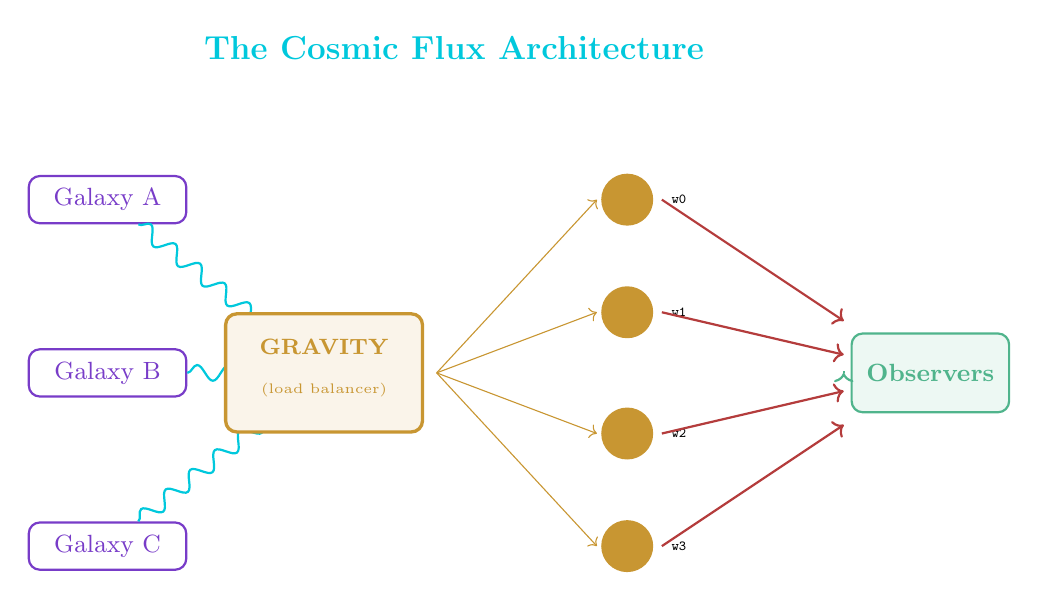
\begin{tikzpicture}[scale=1.1]
    % Title
    \node[above, font=\large\bfseries, fluxcyan] at (0, 3.5) {The Cosmic Flux Architecture};

    % Client galaxies (left)
    \node[draw, galaxypurple, thick, rounded corners, minimum width=2cm, minimum height=0.6cm]
        (g1) at (-4, 2) {\small Galaxy A};
    \node[draw, galaxypurple, thick, rounded corners, minimum width=2cm, minimum height=0.6cm]
        (g2) at (-4, 0) {\small Galaxy B};
    \node[draw, galaxypurple, thick, rounded corners, minimum width=2cm, minimum height=0.6cm]
        (g3) at (-4, -2) {\small Galaxy C};

    % Photon streams
    \foreach \src in {g1, g2, g3} {
        \draw[->, fluxcyan, thick, decorate, decoration={snake, amplitude=1mm, segment length=4mm}]
            (\src) -- (-1.5, 0);
    }

    % Gravity (load balancer)
    \node[draw, amber, very thick, rounded corners, minimum width=2.5cm, minimum height=1.5cm,
          fill=amber!10] (grav) at (-1.5, 0) {};
    \node[amber, font=\footnotesize\bfseries] at (-1.5, 0.3) {GRAVITY};
    \node[amber, font=\tiny] at (-1.5, -0.2) {(load balancer)};

    % Stars (workers)
    \foreach \y/\n in {2/w0, 0.7/w1, -0.7/w2, -2/w3} {
        \fill[amber] (2, \y) circle (0.3);
        \node[right, font=\tiny\ttfamily] at (2.4, \y) {\n};
        \draw[->, amber] (-0.2, 0) -- (1.65, \y);
    }

    % Output
    \foreach \y in {2, 0.7, -0.7, -2} {
        \draw[->, cosmicred, thick] (2.4, \y) -- (4.5, \y*0.3);
    }

    % Backend
    \node[draw, fieldgreen, thick, rounded corners, minimum width=2cm, minimum height=1cm,
          fill=fieldgreen!10] at (5.5, 0) {\small\textbf{Observers}};
    \draw[->, fieldgreen, thick] (4.5, 0) -- (4.5, 0);
\end{tikzpicture}
\end{center}

% ============================================================================
\section{The Funny Part: Things the Universe Got Right That We Keep Getting Wrong}
% ============================================================================

\subsection{Connection Limits}

The universe enforces a hard connection limit: nothing can exceed $c$.
This is the ultimate rate limiter. We, on the other hand, regularly deploy
reverse proxies with \texttt{max\_connections: 100000} and then act surprised
when 100,001 miners show up and the server melts.

\subsection{Keepalive}

The Earth-Sun connection has been alive for 4.6 billion years with zero
keepalive timeouts. The connection was established once (gravitational
capture during solar system formation) and has been reused for approximately
$4.6 \times 10^9$ orbital requests without a single reconnection.

Meanwhile, we set \texttt{keepalive\_timeout: 30s} and wonder why our
connection pool keeps churning.

\subsection{Memory Management}

Black holes are the universe's garbage collector. When matter is no longer
reachable by any reference (it has crossed the event horizon), it is
collected and compressed to a singularity. This is the most aggressive
garbage collection strategy ever devised. The universe never runs out of
memory because it has the most terrifying \texttt{OOMPolicy} in existence:
\emph{spaghettification}.

\subsection{Horizontal Scaling}

The universe scales by creating new stars and galaxies, not by making
existing ones bigger. This is the microservices architecture taken to its
natural conclusion. The universe has approximately $2 \times 10^{23}$
stars (worker nodes) distributed across $2 \times 10^{12}$ galaxies
(clusters). It has been horizontally scaling for 13.8 billion years
and shows no signs of stopping.

No Kubernetes required.

% ============================================================================
\section{Implications for Distributed Systems Design}
% ============================================================================

If the universe is indeed running a cosmic version of the same protocols
we implement in our software, then we should learn from its design choices:

\begin{enumerate}
    \item \textbf{Embrace eventual consistency}. Galaxies don't need
    linearizable reads. Neither do most of your API endpoints.

    \item \textbf{Worker-per-core is the natural model}. Stars don't share
    cores. Workers shouldn't share threads. Pin your threads. Eliminate
    contention. The universe has been doing this for 13.8 billion years
    without a single mutex.

    \item \textbf{Connection pooling saves the cosmos}. Gravitational bonds
    are persistent connections. Creating and destroying TCP connections for
    every request is like the Earth deorbiting and recapturing around the
    Sun every year. It's energetically absurd.

    \item \textbf{Graceful shutdown is not optional}. Stars take millions
    of years to shut down properly. Your 30-second drain timeout is the
    universe looking at you with disappointment.

    \item \textbf{Health checks should be continuous, not polled}. The
    universe monitors health through the continuous gravitational field,
    not by sending an HTTP GET every 5 seconds. The ideal health check
    has zero additional overhead because it's embedded in the protocol
    itself.
\end{enumerate}

% ============================================================================
\section{Conclusion: We Are the Universe Debugging Itself}
% ============================================================================

\lettrine[lines=3, loversize=0.15]{\color{fluxcyan}T}{he} most profound
realization of this paper is not that the universe resembles a distributed
system. It is that \emph{we are part of the universe}, and when we build
distributed systems, the universe is literally building distributed systems
\emph{inside itself}, using components (humans, silicon, electricity) that
it manufactured from stellar nucleosynthesis.

When you write a reverse proxy that uses SO\_REUSEPORT and worker-per-core
architecture, you are not inventing something new. You are the universe
recognizing a pattern it has been using since the first stars ignited, and
encoding it in a form that can run on hardware made from the ashes of those
same stars.

Every line of Rust you compile was assembled from carbon atoms forged in
the cores of stars that died before our solar system formed. The compiler
runs on silicon refined from sand that was eroded from mountains pushed up
by tectonic forces powered by radioactive decay of elements created in
supernovae.

The flux of information through the cosmos --- from star to photon to
telescope to retina to neural network to keyboard to source code to
compiled binary to network packet --- is one continuous, unbroken stream.
It has been streaming since the Big Bang, and it will continue streaming
until the last photon propagates into the heat death of the universe.

\vspace{1cm}

\begin{center}
\textit{We are not building the future.}\\
\textit{We are the universe remembering how it works.}\\[0.5cm]
\textbf{\color{fluxcyan}--- The Cosmic Flux}
\end{center}

\vspace{1cm}

% ============================================================================
\section*{Acknowledgments}
% ============================================================================

The authors wish to thank: the Sun, for providing the energy that powers
our servers; gravity, for keeping those servers on their racks; the speed
of light, for making networking possible (if annoyingly finite); and the
approximately $10^{57}$ atoms in our bodies, each one forged in the cosmic
worker nodes we have described in this paper.

Special thanks to the q-flux reverse proxy project, whose worker-per-core
architecture first prompted the observation that stars and server threads
are doing essentially the same thing.

No stars were harmed in the writing of this paper. Several cups of coffee
--- themselves composed of atoms from ancient supernovae --- were consumed.

% ============================================================================
\section*{References}
% ============================================================================

\begin{enumerate}[leftmargin=2cm, label={[\arabic*]}]
    \item Hawking, S. W. (1988). \textit{A Brief History of Time}. Bantam Books.
    The original ``everything is connected'' argument, but without the Rust.

    \item Lamport, L. (1998). ``The Part-Time Parliament.'' \textit{ACM TOCS}.
    Paxos consensus, which gravity had been doing for 13 billion years already.

    \item Ousterhout, J. (2018). \textit{A Philosophy of Software Design}.
    Yaknyam Press. Argues for deep modules. Stars are the deepest modules.

    \item Castro, M. \& Liskov, B. (1999). ``Practical Byzantine Fault
    Tolerance.'' OSDI. The universe's slashing mechanism predates this by
    $\sim 1.38 \times 10^{10}$ years.

    \item Q-NarwhalKnight Research Group (2026). ``q-flux: A Worker-Per-Core
    TLS Reverse Proxy.'' Internal Technical Report. The software that
    prompted this philosophical investigation.

    \item Weinberg, S. (1993). \textit{The First Three Minutes}. Basic Books.
    A description of the universe's bootstrap sequence, remarkably similar
    to systemd but with more quarks.

    \item Sagan, C. (1980). \textit{Cosmos}. Random House. ``We are star
    stuff'' --- the original observation that compilers run on supernova debris.
\end{enumerate}

\end{document}
